
The contradictory conclusions that arise from the experimental results presented in Figure~\ref{fig:BestWorstComparison} are caused by two issues: (1) the representation of a space of program behaviours by a single point in that space; and (2) the modelling of the effect of uncontrolled variables on the result of the experiments. The use of \CP\ with a leave-one-out evaluation methodology leads to a more appropriate evaluation of the space of behaviour variations due to data input. The repetition of each experiment a reasonable number of times and the reporting of the average of these runs with a corresponding confidence interval to inform about this variation leads to a better accounting for he effect of uncontrolled variables that affect the results of the experiments. The result is a more accurate prediction of performance from the benchmark-based evaluation.

\REM{
This section explains the issues of collecting and analyzing data in the experimental setting. To have a minimum amount of confidence in the values collected it is mandatory to have a strong knowledge of the environment, how much noise could the data possibly have, and how to overcome the difficulties in the measuring process. There is a method to follow and then make sure the data analysis is correct and sound. At first, there is always noise, but the level of the noise will have impact on the number of times an experiment must be repeated; second, after collecting the data the analysis must be carried out, hence as there is noise it is mandatory to show the noise level, showing the values through the use of error bars (for the variance found in the data). Nonetheless this section uses these variance to explain the speedup and slowdown results of \refSection{sec:speedup}.

Every experimental science suffer from the same problem, evaluation of the data already collected. Even the simple idea of collecting data can become a painful task, because the measurement process may introduce errors, or cause distortion in the data.
}

Uncontrolled variables include processes running in background, operating system calls, interruptions, memory allocation, and other sources, including the measurement process itself. Hence, it is important to have a good understanding of the sources of performance disturbances in  the system~\cite{Kalibera2013}.
Kalibera and Jones state that the majority of the experimental studies lack a rigorous statistical methodology~ \cite{Kalibera2013}. A methodology to deal with the effect of uncontrolled variables is to examine the distribution of the data and identify measurements that can safely be eliminated because they are tainted by the effect of uncontrolled variables. For instance, \refFigure{fig:gauss} depicts a scatter plot of $1000$ sequential runs of the program \bzip\  compiled using the \funcname{Static} inliner (\llvm) and run with the {\tt ebooks} input. For \bzip\ and \gzip the code used is not the one distributed by SPEC, but rather fully-functional versions of these programs. Using these versions eliminates the unrealistically-simplified profiling situation where mutually-exclusive use cases are combined into a single program run. Consequently, these programs cannot do decompression and compression, or multiple levels of compression, within the same run.  These distinct use-cases must be covered by different inputs in the program workload.
The inputs for compression include images, ebooks in a variety of formats, movies in MP4 format, textual representation of proteins, audio books, and object files~\cite{BerubePhD}.

\jna{We must state what is the benchmark run to produced the scatter plot shown in Figure \refFigure{fig:gauss} and also what was the input used for those runs.}

\jna{What is our rationalization for concluding that we should see the same pattern of execution for all experiments based on the results shown in Figure \refFigure{fig:gauss}? Have we also done this experiment for other benchmarks and are only showing the result for one? Or are we assuming that the results should generalize because the conditions for all experiments are the same?}

\refFigure{fig:gauss} reveals a gaussian noise around the median plus some outliers that are the result of regular operating system activity. These outliers can safely be filtered out from the data set. They are easily discarded because they are more than one standard deviation above the median.

\jna{Make fonts much bigger in \refFigure{fig:gauss}, also change "runs" to "run" in the horizontal axis because "runs" could be the number of runs represented by a point.}
\begin{figure}
  \centering
  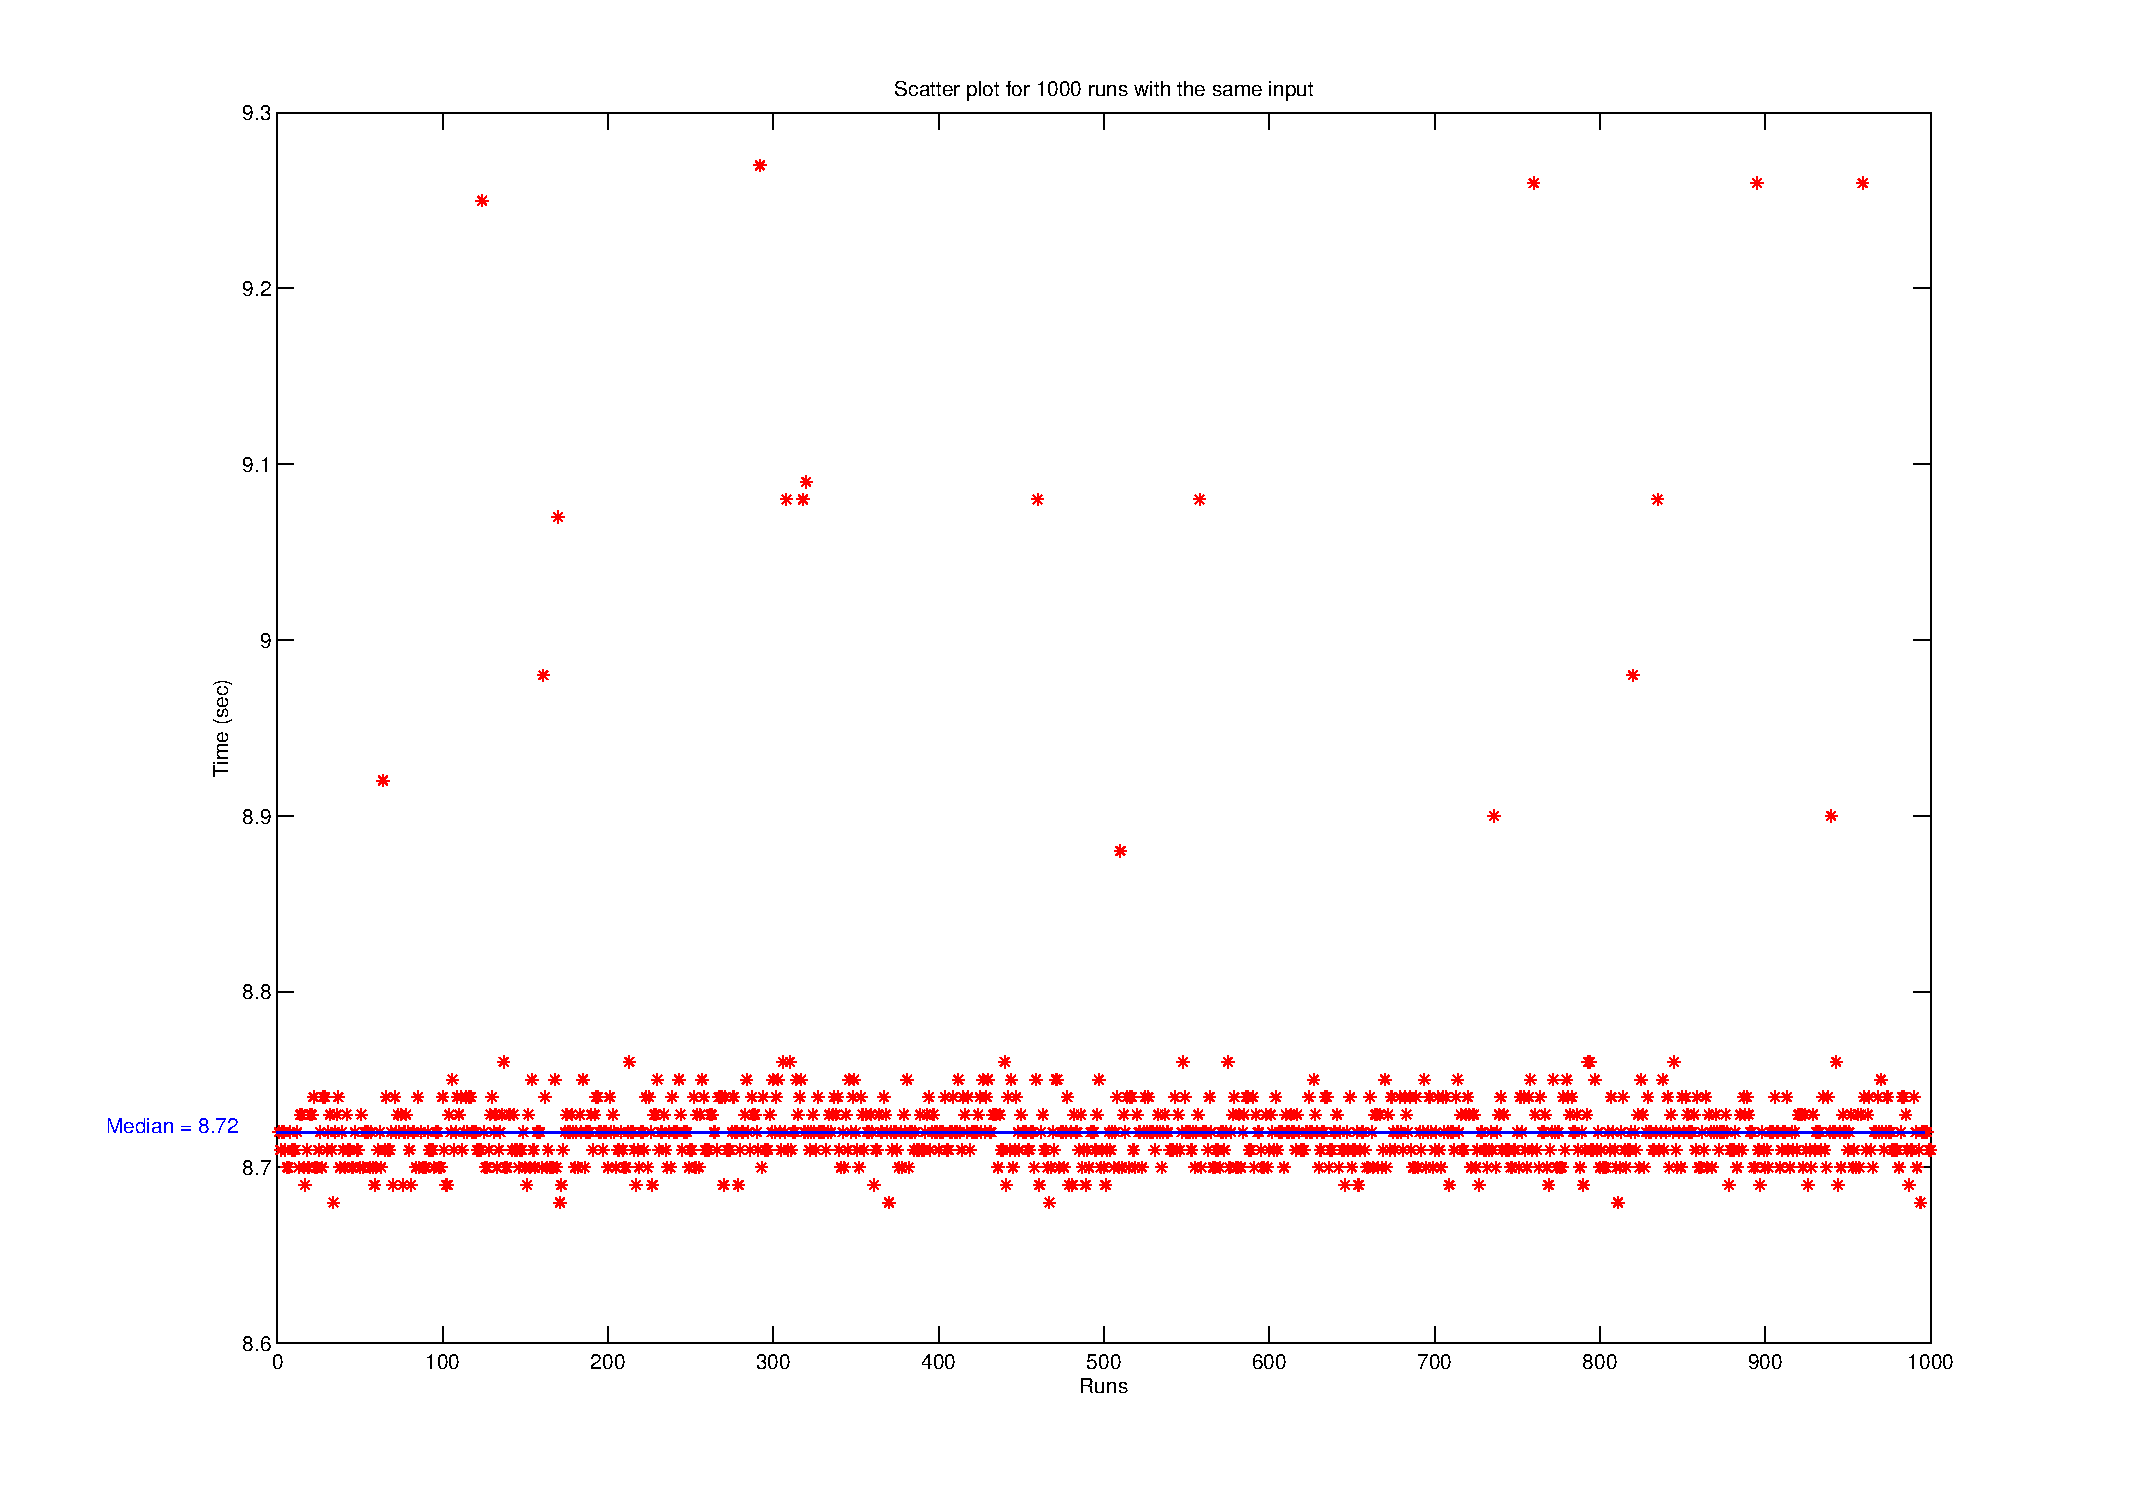
\includegraphics[width=1.00\linewidth]{Figures/nt1000}
  \caption{Scatter plot of the execution times from $1000$ runs of \bzip\ with {\tt ebooks} data input. The execution times appear in the graph in the order in which they were measured.}
  \label{fig:gauss}
\end{figure}

Three independent experiments, with $10$ runs, $100$ runs, and $1000$ runs, reinforces that outliers can be discarded because there is high probability that the measured means have minimum difference among them, and also the behaviour of the program remained unchanged.
\jna{What do these simple statistics tell us?}
Simple statistics --- mean, median, standard-deviation from the mean (std-mean) and standard-deviation from the median (std-median) --- shown in \refTable{tab:robustTest} lead to the conclusion that the three distributions are quite similar. \rlar{completed in response to your comment/question}
\jna{Is this the correct interpretation of the result of the t-tests?}
 Also the results of t-tests run on each sample pairs, and shown in \refTable{tab:ttest}, confirm that the means have high probability of being the same.

\jna{All the captions for all the tables, and graphs, must be rewritten to much more precisely describe what the tables and figures are showing, saying "Simple statistics on the experiment", "t-tests applied pairwise to the $10$, $100$, and $1000$ runs", "Test on the means", etc, is not very helpful. In a good paper, the reader should be able to look at the figure/table, read the caption, and know what is going on without necessarily reading the text.}

\begin{table}
  \centering
  \begin{tiny}
  
\begin{tabular}{lllll}

{\bf Length} & {\bf Mean} & {\bf Median} & 
  {\bf StD Mean} & {\bf StD Median} \\ \hline

10   & 8.7160 & 8.7150 & 0.0100 & 0.0050 \\
100  & 8.7328 & 8.7200 & 0.0187 & 0.0100 \\
1000 & 8.7248 & 8.7200 & 0.0197 & 0.0100 \\

\hline
\end{tabular}

  \end{tiny}
  \caption{Simple statistics on the experiment}
  \label{tab:robustTest}
\end{table}

\jna{We need a clearer and more complete description of the t-tests that were run. Did we run a one-sample or a two-sample t-test? (see http://en.wikipedia.org/wiki/Student's\_t-test). What does the value 0 in all rows of the table mean and how should they be interpreted? Why these p-values prevent us from discarding the null hypothesis? Our logic seems to be that because we did not discard the null hypothesis, we must conclude that the means are similar. Is that a correct reasoning?}

The t-tests in \refTable{tab:ttest} demonstrates that the null hypothesis cannot be discarded, as the value $0$ in each line of the \emph{t-test} column confirms, which means that the three means are similar. The \emph{p-values} show the confidence in the hypothesis, in this case that the means are different. As the values are not high, the confidence is very low.

\begin{table}
  \centering
  \begin{tiny}
  
\begin{tabular}{lllll}

{\bf Runs} & {\bf Reject $H_0$} & {\bf p-value}  \\ \hline

(10-100) & No & 0.3424  \\
(10-1000) & No & 0.6025 \\
(100-1000) & No & 0.1528 \\

\hline
\end{tabular}

  \end{tiny}
  \caption{t-tests applied pairwise to the $10$, $100$, and $1000$ runs}
  \label{tab:ttest}
\end{table}

Another experiment has also shown that the variance when running the same data just three times in a row is not quite different from the one running $100$ times. This experiment was constructed by exercising each `input-run' $3$ times, $3$-consecutive runs for each input, and the whole experiment was run $100$ times% -- which means that the experiment ran $300$ times each input.
A `full-run' in this experiment is a $3$-consecutive run for each input, hence the experiment ran $100$ `full-runs'. Nevertheless the behavior of the system was stressed through the addition of extra noise, simulating an `uncontrolled variable' \cite{Kalibera2013}. The extra noise was injected by the end of the experiment.

The purpose of the extra noise was to verify if the system was robust, even though the effect of the noise can mask the correct values, these data can treated assuring robustness. This way the \CP\ methodology was empirically verified with respect to soundness. As can be seen in \refFigure{fig:CProbust}, the deviation from the mean is not large, and also that there is a subtle knob, which increases the running time of the all programs. It was caused by the execution of another system at the same time competing for the same resources. The running time of each program at each 3-consecutive run can be found in the $y$-axis of \refFigure{CP:ebooks}, and the order number of each full-run is depicted on the $x$-axis. The extra noise can also be visualized in the histogram of \refFigure{CP:hist}, where the $x$-axis depicts the running time for the program and the $y$-axis depicts the number of runs at each bin. These two figures show the $3$-consecutive run for the input data {\tt ebooks}.

\begin{figure}
  \centering
  \begin{minipage}[t]{\linewidth}
    \subfigure[$100$-time runs of the $3$-consecutive execution of input {\tt ebooks} for program \bzip] {
      \begin{minipage}[b]{0.75\textwidth}
        \centering
        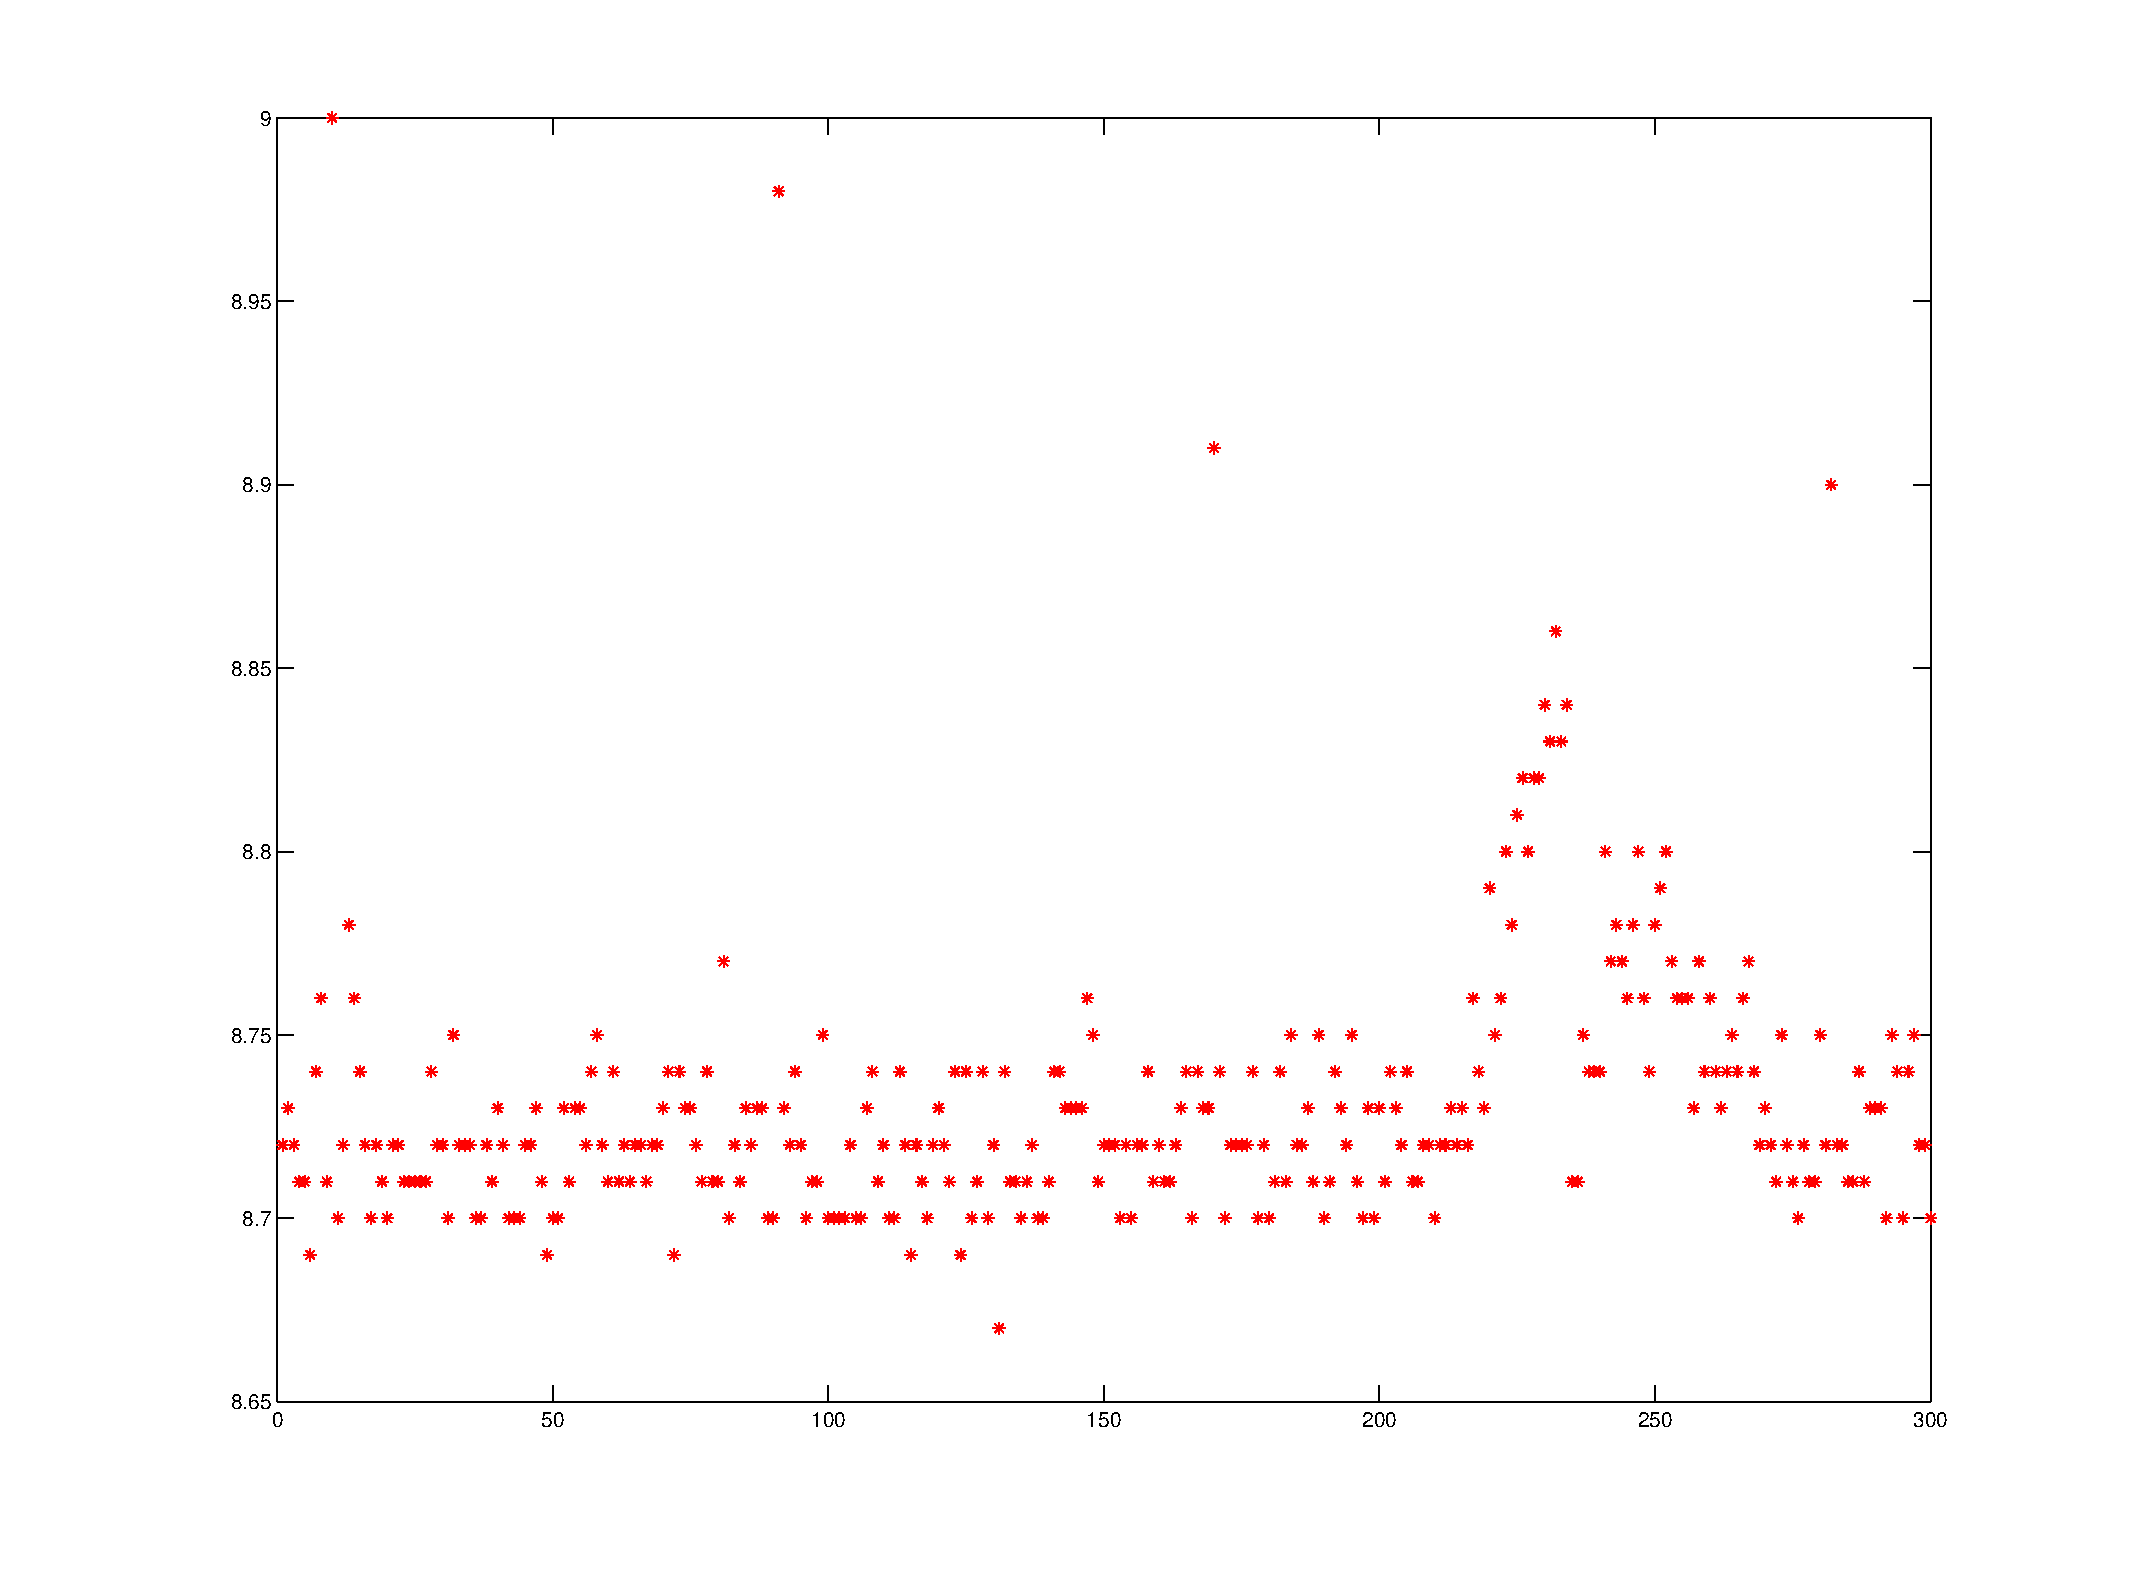
\includegraphics[height=12em]{Figures/ebooks300}
      \end{minipage}
      \label{CP:ebooks}
    }
    \vspace{1em}
    \hrule
    \vspace{1em}
    \subfigure[Histogram for the {\tt auriel} input] {
      \begin{minipage}[b]{0.75\textwidth}
        \centering
        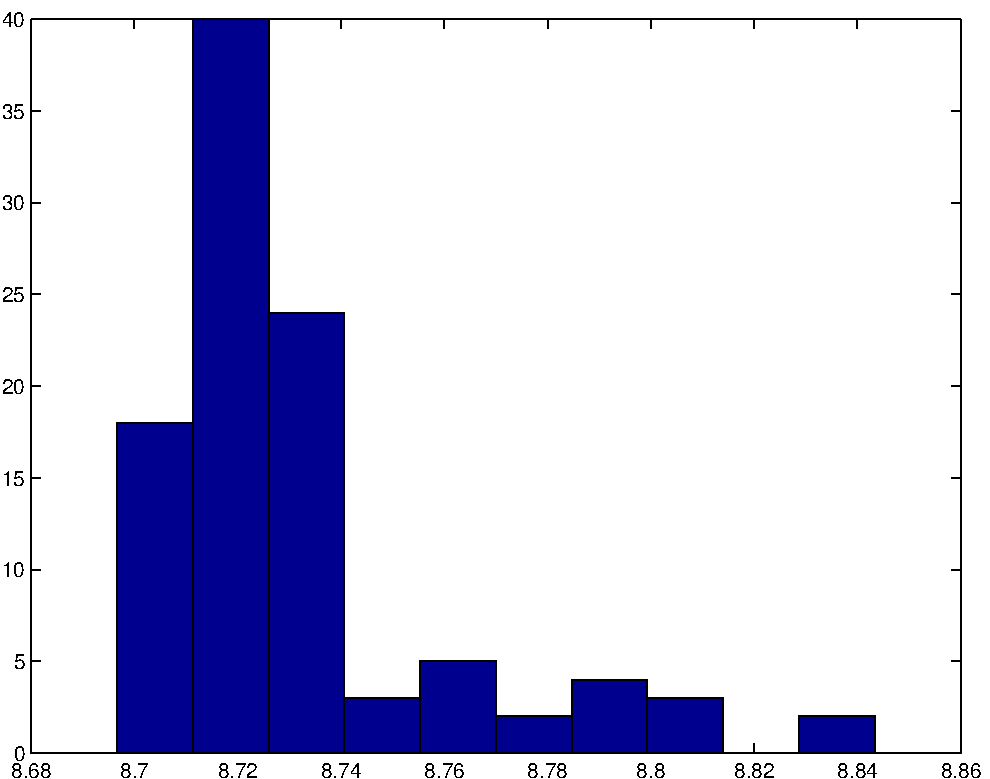
\includegraphics[height=12em]{Figures/ebooks}
      \end{minipage}
      \label{CP:hist}
    }
  \end{minipage}
  \caption{$100$-times running $3$-consecutive experiment}
  \label{fig:CProbust}
\end{figure}

\refFigure{fig:CProbust} and \refFigure{fig:gauss} show that collecting data from single execution can produce erroneous results, even using machines with no other running program. This happens because of the very nature of the empirical experiments, there is some noisy data distribution caused by regular operating system activities, interruption calls, etc. Also, an inclusion of a simple task during the running cycle can perturb the execution time of the program under evaluation, as can be observed by the knob in \refFigure{fig:CProbust}.

The data collected in the experiment are shown in \refTable{tab:simStats}, and the deviations from the mean (and median) to each $3$-consecutive run are summarized as the average, minimum, and maximum values.

\begin{table}
  \centering
  \begin{tiny}
  
\begin{tabular}{lllll}

{\bf Run} & {\bf Mean} & {\bf Median} & 
  {\bf StD Mean} & {\bf StD Median} \\ \hline

1 & 8.7233 & 8.72 & 0.0044   \\
2 & 8.71 & 8.71 & 0.0067 & 0.01   \\
3 & 8.72 & 8.73 & 0.02 & 0.01   \\
4 & 8.7067 & 8.7 & 0.0089 & 0.00   \\
5 & 8.71 & 8.71 & 0.0067 & 0.01   \\
6 & 8.7933 & 8.74 & 0.0778 & 0.01   \\
7 & 8.73 & 8.73 & 0.0067 & 0.01   \\
8 & 8.7233 & 8.71 & 0.0178 & 0.00   \\
9 & 8.73 & 8.73 & 0.0067 & 0.01   \\
10 & 8.7033 & 8.71 & 0.0089 & 0.00   \\
\\
33 & 8.71 & 8.71 & 0.0067 & 0.01   \\
34 & 8.7267 & 8.73 & 0.0044 & 0.00   \\
35 & 8.71 & 8.7 & 0.0133 & 0.00   \\
36 & 8.81 & 8.73 & 0.1133 & 0.01   \\
37 & 8.72 & 8.72 & 0.0133 & 0.02   \\
\\
70 & 8.72 & 8.71 & 0.0133 & 0.00   \\
71 & 8.7133 & 8.72 & 0.0089 & 0.00   \\
72 & 8.7233 & 8.72 & 0.0044 & 0.00   \\
73 & 8.7233 & 8.72 & 0.0044 & 0.00   \\
74 & 8.743333 & 8.74 & 0.0111 & 0.01   \\
75 & 8.7667 & 8.76 & 0.0156 & 0.01   \\
76 & 8.7967 & 8.8 & 0.0111 & 0.01   \\
77 & 8.8133 & 8.82 & 0.0089 & 0.00   \\
78 & 8.83 & 8.83 & 0.0067 & 0.01   \\
79 & 8.8433 & 8.84 & 0.0111 & 0.01   \\
80 & 8.74 & 8.74 & 0 & 0.00   \\
81 & 8.7833 & 8.78 & 0.0111 & 0.01   \\
82 & 8.77 & 8.77 & 0.0067 & 0.01   \\
83 & 8.7667 & 8.76 & 0.0222 & 0.02   \\
84 & 8.79 & 8.79 & 0.0067 & 0.01   \\
85 & 8.7633 & 8.76 & 0.0044 & 0   \\
86 & 8.7533 & 8.76 & 0.0156 & 0.01   \\
87 & 8.7467 & 8.74 & 0.0089 & 0.00   \\
88 & 8.74 & 8.74 & 0.0067 & 0.01   \\
89 & 8.7567 & 8.76 & 0.0111 & 0.01   \\
90 & 8.7267 & 8.72 & 0.0156 & 0.01   \\
91 & 8.71 & 8.71 & 0.0067 & 0.01   \\
\\
92 & 8.7133 & 8.71 & 0.0044 & 0   \\
93 & 8.79 & 8.75 & 0.0733 & 0.03   \\
94 & 8.7167 & 8.72 & 0.0044 & 0   \\
95 & 8.72 & 8.71 & 0.0133 & 0   \\
96 & 8.73 & 8.73 & 0.00 & 0.00   \\
97 & 8.73 & 8.74 & 0.02 & 0.01   \\
98 & 8.73 & 8.74 & 0.02 & 0.01   \\
99 & 8.7133 & 8.72 & 0.0089 & 0   \\
100 & 8.7367 & 8.74 & 0.0178 & 0.02   \\

\hline
\end{tabular}

  \end{tiny}
  \caption{Deviation from the mean and from the median in the experiment}
  \label{tab:simStats}
\end{table}

To confirm that the means are statistically representing the same distribution the t-tests were also run. This is summarized in \refTable{tab:statTest} below. It is easy to see that the number of outliers is little, except for the knob region. 
%because the runtime was being raised during certain amount of time pushing a gradient to increase the time values, and after it, what happened was the other way around, decreasing the time values. Both tables \refTable{tab:simStats} and \refTable{tab:statTest} are shown for the runs.

\begin{table}
  \centering
  \begin{tiny}
  
\begin{tabular}{lllll}

{\bf Runs} & {\bf t-test} & {\bf p-value}  \\ \hline

1 & 0 & 0.706108  \\
2 & 0 & 0.328462  \\
3 & 0 & 0.598565  \\
4 & 0 & 0.259765  \\
5 & 0 & 0.328462  \\
6 & 1 & 0.006947  \\
7 & 0 & 0.938929  \\
8 & 0 & 0.706426  \\
9 & 0 & 0.938929  \\
10 & 0 & 0.201735  \\
\\
33 & 0 & 0.328462  \\
34 & 0 & 0.820524  \\
35 & 0 & 0.328682  \\
36 & 1 & 0.00085  \\
37 & 0 & 0.598316  \\
\\
70 & 0 & 0.598233  \\
71 & 0 & 0.408107  \\
72 & 0 & 0.706108  \\
73 & 0 & 0.706108  \\
74 & 0 & 0.600263  \\
75 & 0 & 0.116071  \\
76 & 1 & 0.003654  \\
77 & 1 & 0.000274  \\
78 & 1 & 0.000013  \\
79 & 1 & 0.000001  \\
80 & 0 & 0.70832  \\
81 & 1 & 0.02056  \\
82 & 0 & 0.085091  \\
83 & 0 & 0.116484  \\
84 & 1 & 0.008985  \\
85 & 0 & 0.154594  \\
86 & 0 & 0.330314  \\
87 & 0 & 0.500169  \\
88 & 0 & 0.708384  \\
89 & 0 & 0.261142  \\
90 & 0 & 0.820684  \\
91 & 0 & 0.328462  \\
\\
92 & 0 & 0.408  \\
93 & 1 & 0.010463  \\
94 & 0 & 0.498166  \\
95 & 0 & 0.598233  \\
96 & 0 & 0.938915  \\
97 & 0 & 0.939012  \\
98 & 0 & 0.939012  \\
99 & 0 & 0.408107  \\
100 & 0 & 0.823099  \\
  
\hline
\end{tabular}

  \end{tiny}
  \caption{Test on the means}
  \label{tab:statTest}
\end{table}

%This kind of experiment can bring confidence in the data collected. In our case it brought confidence in the machine learning method devised to tune-in the inlining parameters of the compiler. 
To obtain low variance one possibility is to increase the number of consecutive runs for each individual input. Nevertheless, these experiments have shown that $3$-consecutive run is a good choice, because it does not penalize much the total running time of the system.

The experiments also have shown that single-run testbeds are error-prone because they don't take the variance into account. The results of an experiment (speedups, or slowdowns) are robust only if there is statistical assurance that the variance on the data is not large.


\subsection{Analyzing the speedup results}

As aforementioned, the actual experiments collected $3$ different run-times for each program at each input, hence it was just a matter of choosing least and greatest values to exhibit a speedup or a slowdown. In a single-run methodology any combination would be plausible to occur.

The complete and correct values are described below. This section end with a figure that was generated by our framework, where the error bars are clearly depicted in it, showing the variance on the speedup geometric means.

\subsubsection{Analysis of\ \ \bzip\  and  \gzip}

After analyzing the inlining environment and having the confidence that the results are trustful, the first program studied was \bzip. Collecting data from the same setup (hardware and software) in $18$ different settings was the first step. \refFigure{fig:fdllrep} shows the data collected. The vertical axis shows the normalized execution geometric mean time for each setting, the baseline is Never (no inlining), and the horizontal axis shows the settings organized by number. The red ``*" represent the normalized geomean time of the \FDI\ inlined program, and the blue ``o" represent the normalized geomean for \llvm\ inlined program.

\begin{figure}
  \centering
  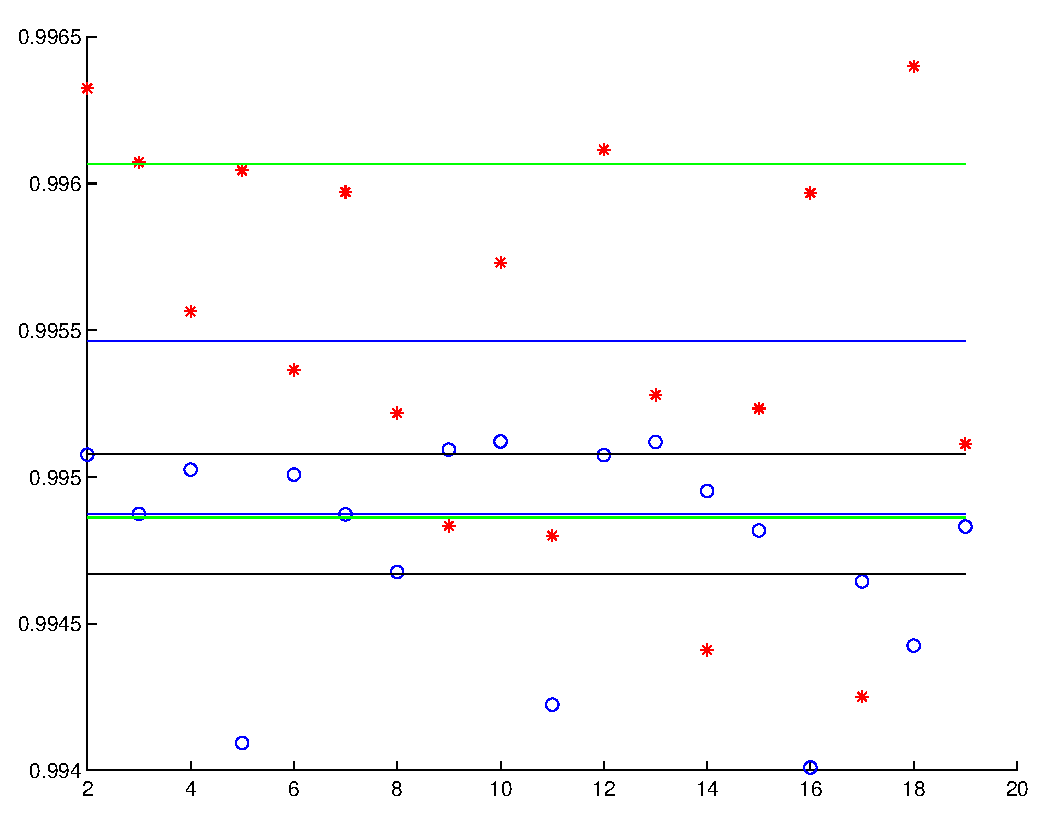
\includegraphics[width=1.00\linewidth]{Figures/fdllrep}
  \caption{The $18$ different settings for \bzip\ of the same setup}
  \label{fig:fdllrep}
\end{figure}

The blue lines in the figure show each median value for the geometric means, the green lines represent one standard deviation from the median for the \FDI\ case, while the black lines represent the standard deviation from the median for the \llvm\ case. As it can be seen, not only the values are too similar, varying only from the fourth decimal digit, but also the medians and their standard deviations overlap, collapse. This is a strong indicator that there is no significant difference between those measures.

Now just consider that a single-run experiment could have measured any one of the $3$-consecutive run values individually, moreover, a single run may have also collected the best, or the worst values for the actual times of the experiment. Hence, to outcome a speedup for \FDI\, the experiment could have collected the worst running time for \llvm\ inlined program, and the best running time for the \FDI\ inlined program.

Even though this biased data showed a speedup, it was really worthless, only $0.46 \%$. Therefore, to reinforce that the input set is also a big issue, the data were "adjusted", leaving the slowdowns and some of the tiny speedups gathered from the set of inputs out of the final list to be shown. This way a tiny, but possibly measurable speedup, was presented in \refSection{sec:speedup}. Nevertheless, defining a list of inputs is an issue and has to be treated as part of the experiment design, as this ``speedup'' have shown. The full data for the "speedup" experiment are shown in table \refTable{tab:fullexp}.

\begin{table}
  \centering
  \begin{tiny}
  
\begin{tabular}{lllll}

{\bf Input} & {\bf Normalized \FDO} & {\bf Normalized \llvm} & {\bf Speedup} \\ \hline

auriel & 0.9720 & 1.0076 & 0.9647   \\ 
avernum & 0.9922 & 0.9905 & 1.0017 \\
cards & 0.9909 & 0.9989 & 0.9919  \\
ebooks & 0.9909 & 0.9920 & 0.9988  \\
gcc & 0.9966 & 1.0059 & 0.9907  \\ 
lib-a & 0.9940 & 0.9970 & 0.9970  \\ 
mohicans & 1.0000 & 1.0048 & 0.9951  \\
ocal & 0.9988 &1.0075 & 0.9913  \\ 
paintings & 1.0000 & 1.0051 & 0.9949  \\
potemkin & 0.9916 & 0.9887 & 1.0029  \\
proteins-1 & 0.9977 & 0.9910 & 1.0068  \\
proteins-2 & 0.9813 & 0.9950 & 0.9862  \\
revelation & 0.9868 & 0.9887 & 0.9980  \\ 
sherlock & 1.0000 & 1.0020 &1.0125  \\ 
usrlib & 1.0000 & 0.9875& 1.0458  \\  \hline
Speedup & & & 0.9953 (0.46 \%) \\

\hline
\end{tabular}

  \end{tiny}
  \caption{Summary of the normalized data used to produce a speedup for \bzip}
  \label{tab:fullexp}
\end{table}

On the other hand, in \refSection{sec:slowdown} the opposite was performed, choosing the worst individual running time for the \FDI\ inlined program and the best running time for the \llvm\ inlined program. Proceeding this way it was easy to present, from "a different" individual measuring, a slowdown. And as both results followed the same methodology, they are both correct, and this is unexplainable unless considering that there is variance on the data collected.

The same process was employed for the \gzip\ case, using $20$ different settings. \refFigure{fig:gzipfdll} presents the \gzip\ data in the same way of \refFigure{fig:fdllrep}. From \refFigure{fig:gzipfdll} there can be seen no evidence of speedup for this setup, and even though a speedup was reported.

\begin{figure}
  \centering
  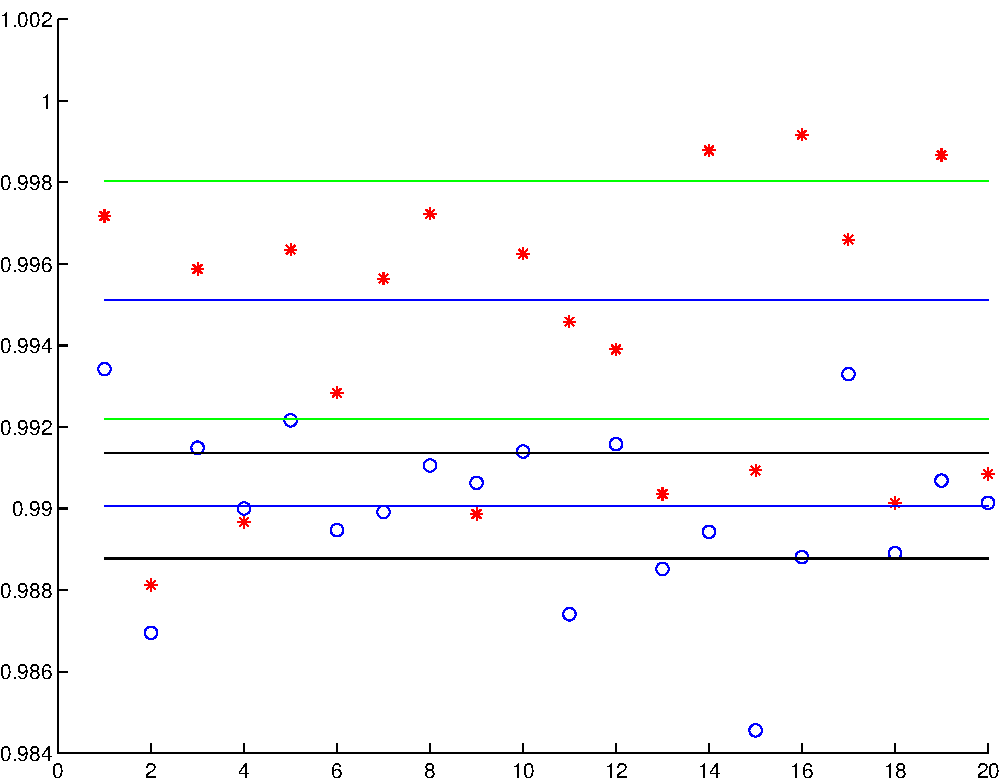
\includegraphics[width=1.00\linewidth]{Figures/gzipfdll}
  \caption{The $20$ different settings for \gzip\ of the same setup}
  \label{fig:gzipfdll}
\end{figure}

Although these cases were artificially constructed from empirical data, if a single-run methodology was employed these results could appear. But employing \CP\ methodology allows a researcher to correctly identify the statistical variance on the data and to discard speedups or slowdowns. This result, in a certain way, reinforces the result of Curtsinger and Berger, reporting no speedup of $-O2$ over $-O3$ for all benchmarks they analyzed, when code randomization is applied~\cite{Curtsinger2013}.

%=============== GOBMK

\subsubsection{Analysis of \gobmk}

For \gobmk\ the input set was chosen in a similar way to that for \bzip\ and \gzip\ cases. The full 15-input set was applied, and if the full input-set is taken, the experiment would have produced a different result, the speedup would be of $1.01 \%$, as shown in \refTable{tab:fullspeedupgbk} and in \refFigure{fig:gobmkall}.

\begin{table}
  \centering
  \begin{tiny}
  
\begin{tabular}{lllll}

{\bf Input} & {\bf \FDO\ normalized} & {\bf \llvm\ normalized} & {\bf Speedup} \\ \hline

13x13 & 0.9922 & 0.9983 & 0.9938  \\
arb & 0.9939 & 0.9969 & 0.9969  \\
arend & 0.9894 & 1.0017 & 0.9877  \\
arion & 0.9934 & 0.9989 & 0.9945  \\
atari_atari & 0.9838 & 1.0000 & 0.9838  \\
buzco & 0.9912 & 0.9970 & 0.9941  \\
connect & 0.9881 & 1.0118 & 0.9766  \\
connection & 0.9881 & 1.0039 & 0.9843  \\
dniwog & 0.9924 & 0.9977 & 0.99470  \\
nicklas2 & 0.9980 & 1.0019 & 0.9960  \\
nicklas4 & 0.9896 & 0.9960 & 0.9936  \\
nngs & 0.9905 & 0.9989 & 0.9915  \\
score2 & 0.9775 & 0.9958 & 0.9816  \\
trevorc & 0.9928 & 1.0004 & 0.9923  \\
trevord & 0.9895 & 1.0025 & 0.9870  \\  \hline

Geomean & & & 0.9899 (1.01 \%)\\
  
\hline
\end{tabular}

  \end{tiny}
  \caption{Summary of the normalized data used to produce a speedup for \gcc}
  \label{tab:fullspeedupgbk}
\end{table}

\begin{figure}
  \centering
  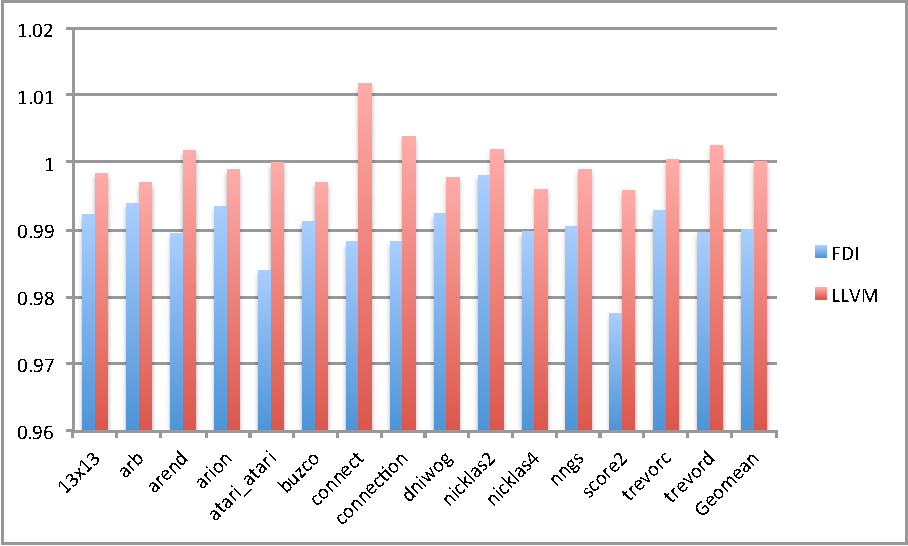
\includegraphics[width=1.00\linewidth]{Figures/speedupgbkall}
  \caption{The complete data of the speedup for \gobmk}
  \label{fig:gobmkall}
\end{figure}

%=============== GCC

\subsubsection{Analysis of \gcc}

For \gcc\ there were two different outcomes, one with the input set chosen, similar to the \bzip, \gzip, and \gobmk\ cases, and another one with a somewhat even more reduced input set, which produced an even better speedup. Again, this was done to raise the question about the proper set of inputs to be employed.

The full 15-input set was applied, and if the full input-set is taken, the experiment would have produced a different result, the speedup would be of $2.52 \%$, as shown in \refTable{tab:fullspeedup} and in \refFigure{fig:gccall}.

\begin{table}
  \centering
  \begin{tiny}
  
\begin{tabular}{lllll}

{\bf Input} & {\bf \FDO\ normalized} & {\bf \llvm\ normalized} & {\bf Speedup} \\ \hline

166 & 0.9494 & 0.9733 & 0.9754  \\
200 & 0.9617 & 0.9735 & 0.9879  \\
c-typeck & 0.9097 & 0.9745 & 0.9335  \\
cccp & 0.9650 & 0.9700 & 0.9948  \\
Cp-decl & 0.9554 & 0.9849 & 0.9700  \\
expr & 0.9035 & 0.9552 & 0.9458  \\
expr2 & 0.8630 & 0.9660 & 0.8934  \\
g23 & 0.9119 & 0.9849 & 0.9259  \\
integrate & 0.9811 & 1.0251 & 0.9570  \\
s04 & 0.9886 & 1.0181 & 0.9710  \\
scilab & 0.9945 & 1.0043 & 0.9902  \\
bzipR-all & 0.9870 & 1.0092 & 0.9780  \\
lbm-all & 0.8888 & 1.0000 & 0.8888  \\
mcf-all & 0.9487 & 1.0000 & 0.9487  \\
parser-all & 0.9945 & 1.0364 & 0.9596  \\
Geomean & & & 0.9541 \\
  
\hline
\end{tabular}

  \end{tiny}
  \caption{Summary of the normalized data used to produce a speedup for \gcc}
  \label{tab:fullspeedup}
\end{table}

\begin{figure}
  \centering
  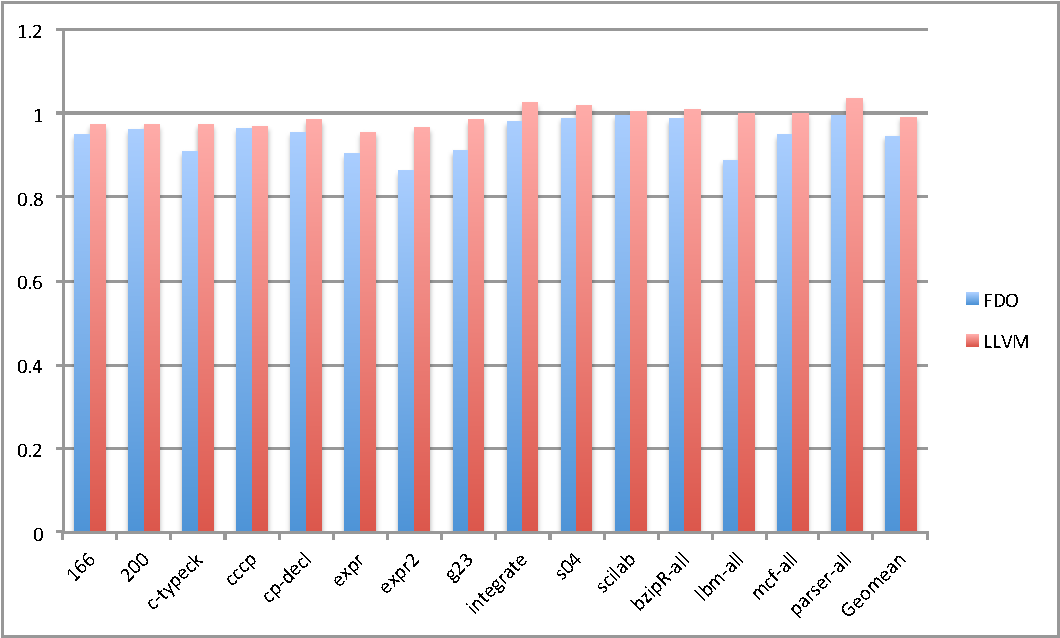
\includegraphics[width=1.00\linewidth]{Figures/speedupgccall}
  \caption{The complete data of the speedup for \gcc}
  \label{fig:gccall}
\end{figure}

\jna{Must explain \refFigure{fig:gcc-results}  in its entirety. Must explain what each point represent (see Berube's thesis). Also must explain $\mu_g$ Execution Time on the vertical axis.}
The evaluation of inlining used fourteen different reward functions for the combined-profiling inlining (see \refFigure{fig:gcc-results}). The normalized execution time for each of those reward functions uses a 3-fold cross-validation. For instance, to obtain the {\tt single} measurement in the figure, for each input $u$ in the workload $\cal{W}$, $u$ is used for training and the generated program is tested using a leave-one-in methodology, {\em i.e.} the execution times for all inputs in $\cal{W}$ except $u$ is obtained, and the speedup for each of these times in relation to the baseline is computed. then the geometric average of these speedups is computed. each of these times is

$\mu_g(\Wfull)$ is the geometric mean of normalized execution
  times for \Wfull, measured by 3-fold cross-validation:
  $$ \mu_g(\Wfull) =  \sqrt[|\Wfull|]{\prod_{i \in \Wfull} \frac{t_u(i)}{\blt{i}}}
  $$
	
Where
$t_u(i)$ is the execution time of an \FDO\ version of a program
  on input $i$ when $u$ is used as the training workload, and $\blt{i}$ is the execution time for the baseline \Never\ running on input $i$. Both $t_u(i)$  and $\blt(i)$ are  measured as the average
  of three runs.

$\tau_u(i) = \frac{\blt{i}}{t_u(i)}$.

Therefore, the input-set matters, as much as a sound methodology. To summarize this section and illustrate the outcomes of the framework employing \CP\ methodology, \refFigure{fig:gcc-results} presents one of the figures automatically generated by the framework. In this figure it can be observed that there was no speedups, nor slowdowns for the \gcc\ case, the error bars present in \refFigure{fig:gcc-results} demonstrates the level of confidence in the geometric mean results.

This figure reflects the geometric mean of all inputs for one single-run \FDI\ inliner (called single in the figure), twelve different \FDI\ inliners, the \llvm\ inliner (called static in the figure) and another static inliner called benefit.

\begin{figure}
  \centering
  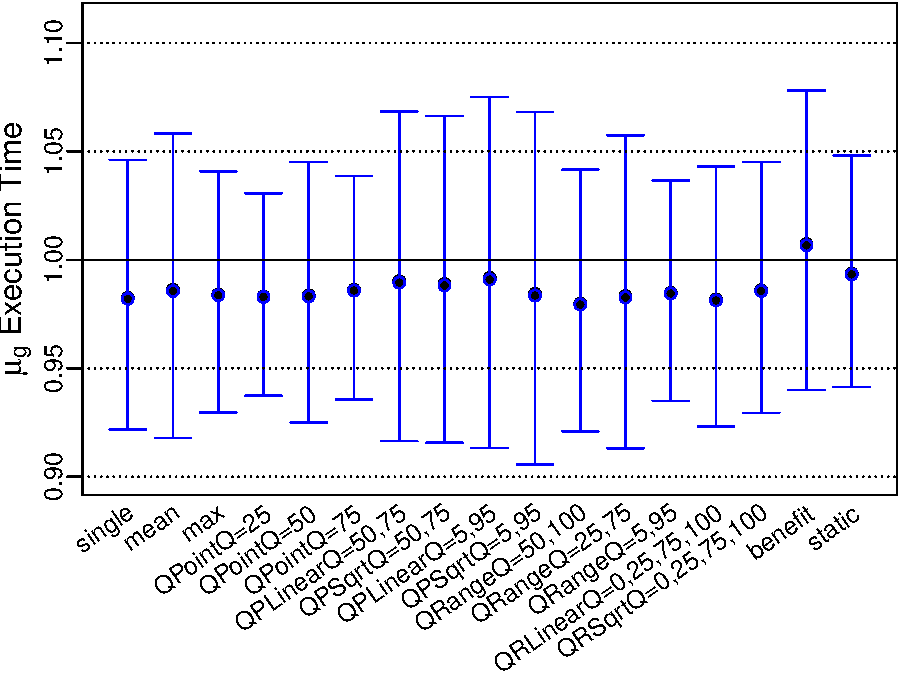
\includegraphics[width=1.00\linewidth]{Figures/gcc-results}
  \caption{The actual result for \gcc\ returned by our \CP\ framework}
  \label{fig:gcc-results}
\end{figure}

%============ regular text

Next section (\refSection{sec:cmbprof}) describes the \CP\ methodology in more detail, explaining its use and how to measure the results, in order to avoid the problems highlighted by the example in \refSection{sec:speedup}.
